%%%%%%%%%%%%%%%%%%%%%%%%%%%%%%%%%%%%%%%%%%%%%%%%%%%%%%%%%%%%%%%%%%%%%%%%%%%%%%%%%%
\begin{frame}[fragile]\frametitle{}
\begin{center}
{\Large Theory: How it works?}
\end{center}
\end{frame}


%%%%%%%%%%%%%%%%%%%%%%%%%%%%%%%%%%%%%%%%%%%%%%%%%%%%%%%%%%%%%%%%%%%%%%%%%%%%%%%%%%
\begin{frame}[fragile]\frametitle{How Mind and Memory Work}
    \begin{columns}
        \begin{column}{0.48\textwidth}
			\begin{itemize}
				\item In typical awake states:
					\begin{itemize}
						\item Sense organs send signals to the conscious mind.
						\item Conscious mind decides what information to relay to the brain.
						\item The brain processes, references memories, and creates responses or stores knowledge.
					\end{itemize}
				\item In sleep:
					\begin{itemize}
						\item Only critical or threatening signals are relayed.
						\item Subconscious mind remains active, processing memories without conscious interference.
					\end{itemize}
			\end{itemize}
        \end{column}
        \begin{column}{0.48\textwidth}	
			  \begin{center}
				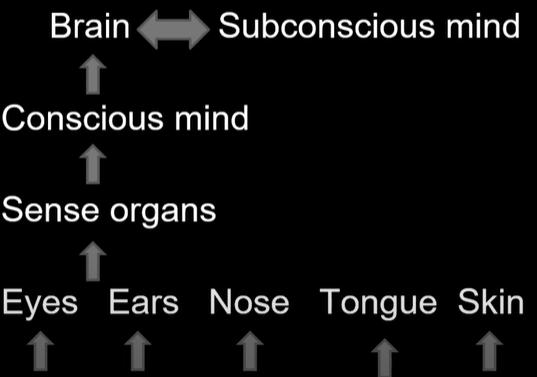
\includegraphics[width=\linewidth,keepaspectratio]{yoganidra14}

				{\tiny (Ref: Yoga Nidra as Therapy - Yogapointindia)}		
				\end{center}	
        \end{column}
    \end{columns}				
\end{frame}

%%%%%%%%%%%%%%%%%%%%%%%%%%%%%%%%%%%%%%%%%%%%%%%%%%%%%%%%%%%%%%%%%%%%%%%%%%%%%%%%%%
\begin{frame}[fragile]\frametitle{Changes in Yoganidra: Bypassing the Brain}

    \begin{columns}
        \begin{column}{0.48\textwidth}
			\begin{itemize}
				\item In Yoganidra:
					\begin{itemize}
						\item The conscious mind bypasses usual processes, directly influencing the subconscious.
						\item Desired affirmations or resolutions can overwrite or reprogram unwanted memories.
						\item This bypass allows deeper, lasting personal transformation without mental resistance.
					\end{itemize}
				\item Conscious instructions integrate seamlessly into the subconscious, enabling habit or perception changes.
			\end{itemize}
        \end{column}
        \begin{column}{0.48\textwidth}	
			  \begin{center}
				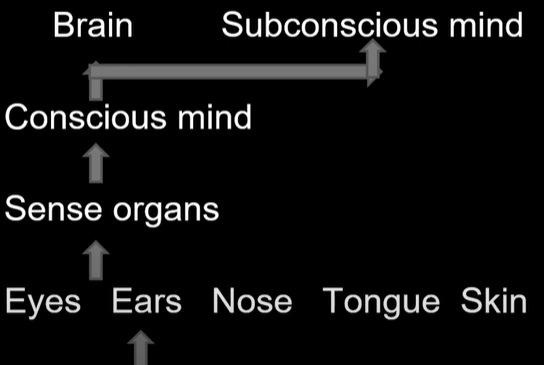
\includegraphics[width=\linewidth,keepaspectratio]{yoganidra15}

				{\tiny (Ref: Yoga Nidra as Therapy - Yogapointindia)}		
				\end{center}	
        \end{column}
    \end{columns}	
	

\end{frame}

%%%%%%%%%%%%%%%%%%%%%%%%%%%%%%%%%%%%%%%%%%%%%%%%%%%%%%%%%%%%%%%%%%%%%%%%%%%%%%%%%%
\begin{frame}[fragile]\frametitle{Swami Rama’s Demonstration of Yoganidra}
    \begin{itemize}
        \item Swami Rama, in Yoganidra, demonstrated heightened awareness by recounting discussions held while he was in a deep sleep state.
        \item This phenomenon indicates awareness in \textbf{delta wave states}, typical of deep sleep but with conscious recollection.
        \item Delta state in Yoganidra aligns with the Turya state: deep rest with expanded consciousness.
    \end{itemize}
\end{frame}

%%%%%%%%%%%%%%%%%%%%%%%%%%%%%%%%%%%%%%%%%%%%%%%%%%%%%%%%%%%%%%%%%%%%%%%%%%%%%%%%%%
\begin{frame}[fragile]\frametitle{The State of Turya in Mandukya Upanishad}
    \begin{itemize}
        \item Turya is the fourth state beyond wakefulness, dreaming, and deep sleep.
        \item It combines elements of deep sleep (rest, rejuvenation) with a keen alertness.
        \item \textbf{In Yoganidra}, practitioners enter Turya, accessing latent aspects of the mind, fostering self-awareness and calm.
    \end{itemize}
\end{frame}



%%%%%%%%%%%%%%%%%%%%%%%%%%%%%%%%%%%%%%%%%%%%%%%%%%%%%%%%%%%
\begin{frame}[fragile]\frametitle{Introduction to Yoga Nidra}
    \begin{itemize}
        \item Overview of the Yoga Nidra steps and how to design it for self-practice or teaching.
        \item Includes essential and optional steps: \textbf{Settling and Internalization, Sankalpa, Body Rotation, Breath Awareness, Opposites, Visualization, Repeating Sankalpa, and Externalization}.
    \end{itemize}
\end{frame}

%%%%%%%%%%%%%%%%%%%%%%%%%%%%%%%%%%%%%%%%%%%%%%%%%%%%%%%%%%%
\begin{frame}[fragile]\frametitle{Stage 1: Settling \& Internalization}
    \begin{itemize}
        \item Essential for all Yoga Nidra practices.
        \item Body preparation in Shavasana (or alternate comfortable positions).
        \item Focus on relaxing body parts, awareness of sensations, and external sounds.
        \item Gradual shift to sound of breath, preparing for inward focus.
    \end{itemize}
\end{frame}

%%%%%%%%%%%%%%%%%%%%%%%%%%%%%%%%%%%%%%%%%%%%%%%%%%%%%%%%%%%
\begin{frame}[fragile]\frametitle{Stage 2: Sankalpa (Resolve)}
    \begin{itemize}
        \item Optional but highly beneficial for personal growth and positive reinforcement.
        \item A short, positive mental statement set at the beginning and repeated at the end.
        \item Sows a seed of intention in the subconscious, helping to reshape personality.
    \end{itemize}
\end{frame}

%%%%%%%%%%%%%%%%%%%%%%%%%%%%%%%%%%%%%%%%%%%%%%%%%%%%%%%%%%%
\begin{frame}[fragile]\frametitle{Stage 3: Rotation of Consciousness}
    \begin{itemize}
        \item Essential step that involves mental awareness of body parts.
        \item No physical movement; focus moves systematically from one part to another.
        \item Consistent pace, starting with the right thumb, concluding with left toe.
        \item Supports relaxation and subconscious awareness.
    \end{itemize}
\end{frame}

%%%%%%%%%%%%%%%%%%%%%%%%%%%%%%%%%%%%%%%%%%%%%%%%%%%%%%%%%%%
\begin{frame}[fragile]\frametitle{Stage 4: Awareness of Breath}
    \begin{itemize}
        \item Focuses on natural breath awareness without altering it.
        \item Can involve counting breaths or observing the breath at various points.
        \item Promotes deeper relaxation and healing by balancing body energy.
    \end{itemize}
\end{frame}

%%%%%%%%%%%%%%%%%%%%%%%%%%%%%%%%%%%%%%%%%%%%%%%%%%%%%%%%%%%
\begin{frame}[fragile]\frametitle{Stage 5: Opposites (Sensations \& Feelings)}
    \begin{itemize}
        \item Optional, focuses on pairs of opposite sensations (e.g., heat/cold, heavy/light).
        \item Harmonizes brain hemispheres, controls unconscious functions, builds emotional resilience.
        \item Brings deep relaxation through catharsis.
    \end{itemize}
\end{frame}

%%%%%%%%%%%%%%%%%%%%%%%%%%%%%%%%%%%%%%%%%%%%%%%%%%%%%%%%%%%
\begin{frame}[fragile]\frametitle{Stage 6: Visualization}
    \begin{itemize}
        \item Optional stage using powerful imagery (e.g., landscapes, symbols).
        \item Draws subconscious content into conscious awareness, aiding self-discovery.
        \item Encourages relaxation by processing deep, often unrecognized emotions.
    \end{itemize}
\end{frame}

%%%%%%%%%%%%%%%%%%%%%%%%%%%%%%%%%%%%%%%%%%%%%%%%%%%%%%%%%%%
\begin{frame}[fragile]\frametitle{Stage 7: Repeating the Sankalpa}
    \begin{itemize}
        \item Optional but recommended if introduced in Stage 2.
        \item Reinforces positive intention as a “seed” planted at the beginning and “watered” at the end.
        \item Enables personality transformation by embedding the resolve into the subconscious.
    \end{itemize}
\end{frame}

%%%%%%%%%%%%%%%%%%%%%%%%%%%%%%%%%%%%%%%%%%%%%%%%%%%%%%%%%%%
\begin{frame}[fragile]\frametitle{Stage 8: Externalization}
    \begin{itemize}
        \item Essential final stage, transitioning back to waking state.
        \item Gradually reconnects awareness from subtle inward focus to physical body and surroundings.
        \item Can include gentle movements and \textbf{Om} chanting for a smooth return.
    \end{itemize}
\end{frame}